\documentclass[aps,pre,amssymb,amsmath,twocolumn,floatfix]{revtex4-2}
\usepackage{graphicx}
\usepackage{amsmath}
\usepackage{dcolumn}
\usepackage{bm}

\graphicspath{ {./img/} }
\bibliographystyle{unsrt}     %% [number]
\renewcommand{\bibname}{Bibliography}

\begin{document}

\title{[NO NAME ARTICLE]}

\author{Ilya Pchelintsev}
\author{Kamilla Faizullina}
\author{Evgeni Burovski}
\affiliation{HSE University, 101000 Moscow, Russia}


% абстракт и введение я напишу немного позже, когда будет более полное
% осмысление работы

\begin{abstract}
    This is an abstract and that's really abstract.
\end{abstract}

\maketitle

\section{Introduction}
This is cite-checking.\cite{Papale2018}

\section{Models and Methods}
In the paper we consider several models: the first one is Ising model on interacting self-avoiding walk from the \cite{faizullina2021critical}, on three different lattices: 2D-square lattice, 3D-square lattice and 2D-triangle lattice. The main difference between square and triangle lattice in defining two additional diagonal monomers on lattice as nearest too, see [FIGURE FOR 2D-SQUARE AND 2D-TRIANGLE LATTICE]. Considering the case of lack of outer magnetic field in this work, the Hamiltonian of the model of fixed conformation $u$ with length $N$ and strength of nearest-neighbors interaction $J$ reads:

\begin{figure}[h!]
\begin{minipage}{0.45\columnwidth}
    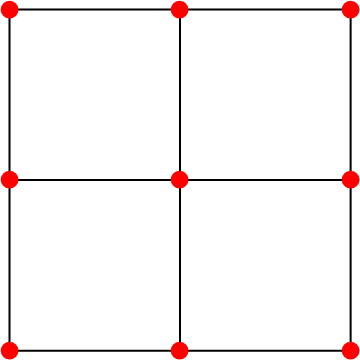
\includegraphics[width=\textwidth]{Images/SqLattice.png}
    \caption{Connections of nearest neighbors interaction in two-dimensional square lattice}
    \label{fig:ISAW_A_J_Zoom}
\end{minipage}
\hfill
\begin{minipage}{0.45\columnwidth}
    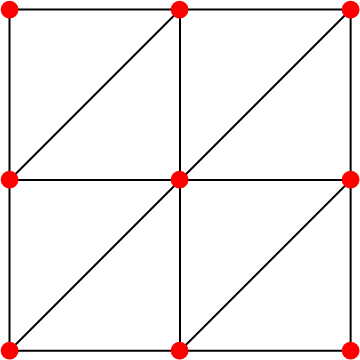
\includegraphics[width=\textwidth]{Images/TriLattice.png}
    \caption{Connections of nearest neighbors interaction in two-dimensional triangular lattice}
    \label{fig:Is_A_J_Zoom}
\end{minipage}

\end{figure}

\begin{equation}\label{H_Ising_ISAW}
  H_{u, N, \{\sigma\}} = - \sum_{\langle i,j \rangle} J  \sigma_{i}  \sigma_{j},\ \ i,j \in u,\ |u| = N
\end{equation}

The summation runs through spins involved in conformation and only with the nearest neighbors. 

The second model considered in this paper is the Ising model on the rectangular lattice from the \cite{Selke2006}. Simulated lattices has $L \times rL$ spins and the Hamiltonian is calculated through interaction between all spins and their nearest neighbors respectively:

\begin{equation}\label{H_Ising_Rectan}
  H_{L, r, \{\sigma\}} = - \sum_{\langle i,j \rangle} J  \sigma_{i}  \sigma_{j}
\end{equation}

Here the $i$-th spin of the lattice has a pair of coordinates from $[1..L] \times [1..rL]$, so $j$-th spin can be called nearest neighbor in square or rectangular lattice, if one of the following conditions are true:

\begin{equation*}
\centering
    \begin{cases}
    x_{i} = x_{j} \\
    |y_{i} - y_{j}| = 1\\
    \end{cases} 
    \begin{cases}
    y_{i} = y_{j} \\
    |x_{i} - x_{j}| = 1\\
    \end{cases} 
\end{equation*}

For comparing magnetic properties of models with similar geometric ones we also define shape factors, such as gyration tensor \cite{Caracciolo_2011}:

\begin{equation}\label{eq:Ten_G1}
    Q_{N,\alpha\beta} = \frac{1}{N+1} \sum^{N}_{i=0}(w_{i,\alpha} - w_{c, \alpha})(w_{i,\beta} - w_{c, \beta})
\end{equation}

where $N$ is length of the system (number of monomers in conformations of Ising-ISAW models and number of spins in the lattice in rectangular Ising), and  $\alpha,\beta$ are coordinates (so, $Q_{N, xx}$ and $Q_{N,yy}$ can be defined as mean squares of coordinates of the points of the model in the cartesian coordinate system with the center in the center of model). Eugen values $q1$, $q2$ of given tensor can be interpreted as $Q_{N, xx}$ and $Q_{N,yy}$ in the coordinate system of eugen vectors, or more important - as square of semi-axes of ellipse of inertia of given system. The proportion of them for systems with length $N$ will be\cite{Caracciolo_2011}: 

\begin{equation}
    r = \sqrt{\frac{\langle q_{1}\rangle_{N}}{\langle q_{2} \rangle_{N}}}
\end{equation}

Eugen values $q1$, $q2$ are also used in enumerating another important shape factor - mean asphericity\cite{Caracciolo_2011}:

\begin{equation}
\label{eq:Asphericity}
    \mathcal{A} = \left\langle \frac{(q_{1} - q_{2})^{2}}{(q_{1} + q_{2})^{2}} \right\rangle_{N}
\end{equation}

% Здесь хочу добавить два графика - прямоугольника и случайного блуждания
% с соответствующими им эллипсами инерции - попробую сделать так чтобы они
% имели одинаковую асферичность - чтобы была ясна задумка первого сюжета

The compared magnetic property of our models is the fourth order cumulant of the magnetization of the Binder cumulant, defined as\cite{Selke2006}:

\begin{equation}
\label{eq:Cumulant}
U_{4} = 1 - \frac{\langle m^{4} \rangle}{3 \langle m^{2} \rangle^{2}}
\end{equation}

Where $\langle m^{4} \rangle$ and $\langle m^{2} \rangle$ are mean fourth and second order of mean magnetization per spin respectively.

We also need to define mean proportion of monomers with fixed number $i$ of nearest neighbors $\langle n_{i} \rangle$, which is counted directly for every monomer in every simulated conformation of walk.

We are interested in comparing models in their respective critical regions. For each structure, critical temperatures of Ising models are known as \cite{Foster2021,Selke2006}:

\begin{table}[h]
    \centering
    \begin{tabular}{|c|c|c|}
        \hline
        Type of lattice & $T_{c}$ \\ \hline
        2D-square & $1.199 \pm 0.003$\cite{Foster2021} \\ \hline
        3D-square & $1.90 \pm 0.02$\cite{Foster2021}\\ \hline
        Rectangular & 2.26918...\cite{Selke2006}\\ \hline
    \end{tabular}
    \caption{Known values of critical temperature of different modifications of Ising-ISAW model and normal Ising on the rectangular lattice}
    \label{tab:Ising_T_c}
\end{table}

% сюда немного позже добавлю критические значения для модели SAW

% Стоит ли добавлять рисунок шага алгоритма 
% и более подробное объяснение методов?? Поскольку ничего не было добавлено, % я решил не расписывать, но описание методов получилось крайне немногословным))


% на самом деле, мне ещё не до конца понятно, какую часть теории достаточно
% просто добавить ссылкой, а что лучше добавить подробным разъяснением

\section{Results}

\subsection{Mean Asphericity and Critical Cumulant}

% если я правильно понимаю, данную подсекцию можно полностью взять из отчёта
% (9.6), как раз данная часть больше всего похожа по содержанию на Results -
% план действий (какие длины были взяты, под какую модель и т.д.), описания
% графиков, таблицы; только с заключением вопрос - его стоит добавить в 
% условный Conclusions или рассужждения о результате желательны здесь же 
% перед частью Bulk.

%пока только рисунки, для хронологии
%более подробное объяснение добавлю позже

We attempted to learn how magnetic properties of Ising-like models depend on their geometrical ones and to define their comparability in critical region, where observable values of models don't depend on the length of conformation $N$. The idea is to compare critical cumulants $U_{4}$ \eqref{eq:Cumulant} of both models of Ising having equal asphericities. Both models are considered to have open boundary conditions (OBC). As we know, in the Ising model on rectangular lattice shape factors like aspect ratio $r$ are the parameters, not observable values. Therefore, we can find \eqref{fig:A_r} value of the aspect ratio of lattice for any asphericity $\mathcal{A}$ \eqref{eq:Asphericity}. Moreover, we know that value of Binder cumulant in Rectangular Ising\cite{Selke2006} in critical region depends on aspect ratio $r$. % добавить графики зависимости значений кумулянта от R%. 
\begin{figure}[h]
    \centering
    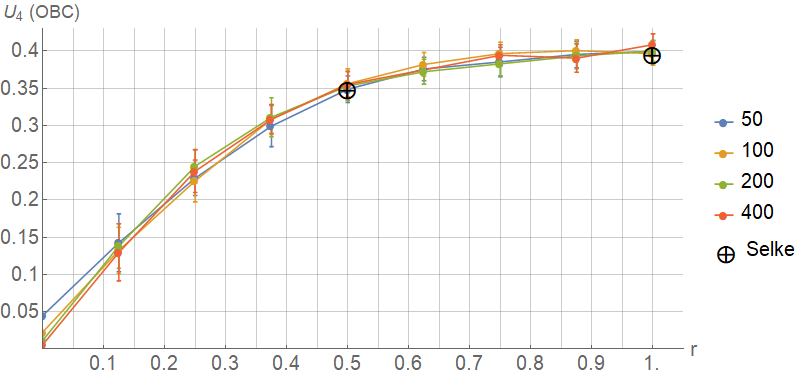
\includegraphics[width=\columnwidth]{Images/CumulantOBC.png}
    \caption{Critical cumulant $U_{4}$\eqref{eq:Cumulant} of Ising model on a rectangular lattice with open boundary conditions as function of aspect ratio $r$ with side length $L$ = 50 (blue), 100 (yellow), 200 (green) and 400 (red). Black markers define values from \cite{Selke2006}}
    \label{fig:A_r}
\end{figure}

\begin{figure}[h]
    \centering
    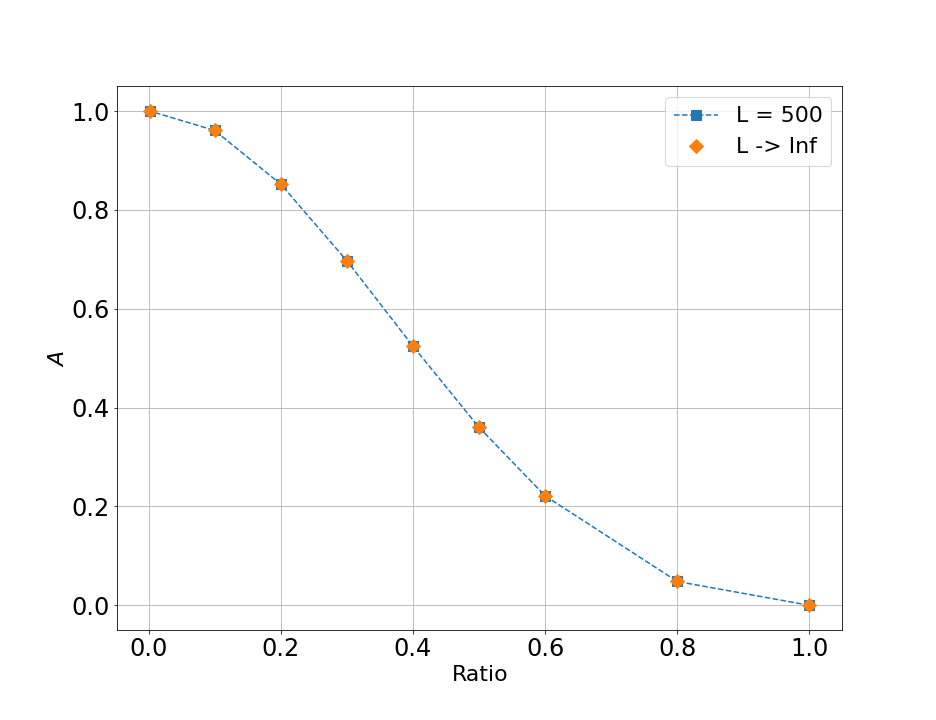
\includegraphics[width=\columnwidth]{Images/A_r.png}
    \caption{Asphericity as function of aspect ratio $r$ of the rectangular lattice with side length = 500 and approximate values for rectangular lattice with infinitely long side}
    \label{fig:A_r}
\end{figure}

% следует ли добавить расчёты оценки зависимости асферичности 
% прямоугольника от стороны? Или это лучше добавить в models and methods?

\begin{figure}[h!]
    \centering
    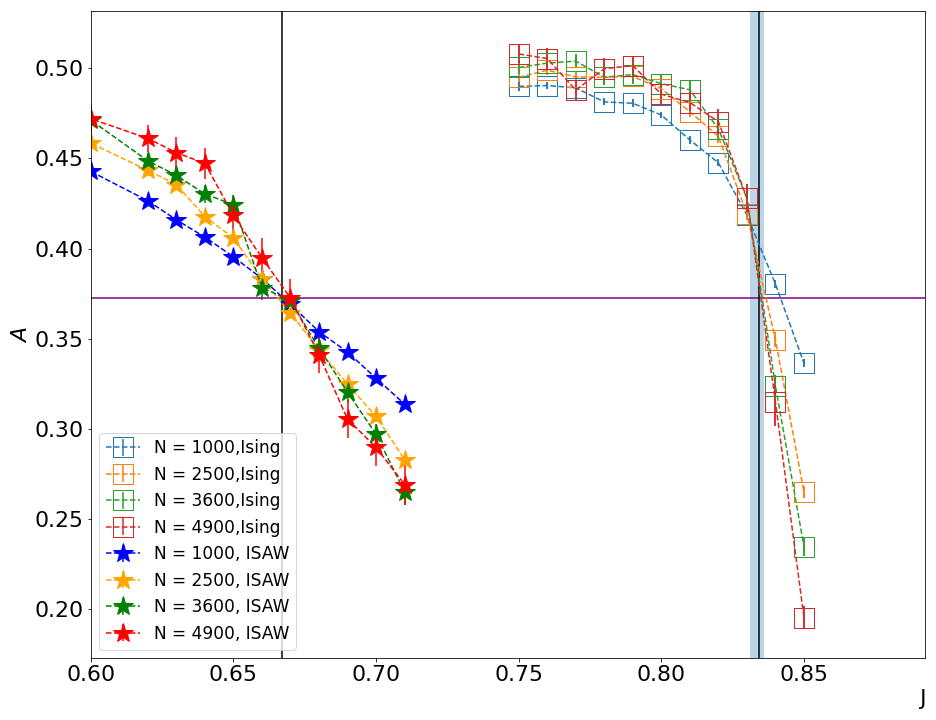
\includegraphics[width=\columnwidth]{Images/Ising_ISAW_A_J_Full.png}
    \caption{Asphericity of Ising-ISAW (empty squares) and ISAW-only models (stars) as function of $J=1/T$, varying lengths of conformations $N$ = 1000 (blue), 2500 (yellow), 3600 (green) and 4900 (red)}
    \label{fig:Ising&ISAW_A_J}
\end{figure}

We enumerated values of asphericity \eqref{eq:Asphericity} of Ising-ISAW model on 2D-square lattice in its critical region \ref{tab:Ising_T_c} for lengths N = 1000-4900. For simulations of this model we used method described in \cite{faizullina2021critical}. Vertical lines on figures define borders (according to statistical errors of known values\ref{tab:Ising_T_c}) of critical regions of Ising-ISAW (red lines) and ISAW models (black line). Horizontal line define value of critical asphericity of ISAW model, which is known from \cite{Caracciolo_2011}.

\begin{figure}[h!]
    \centering
    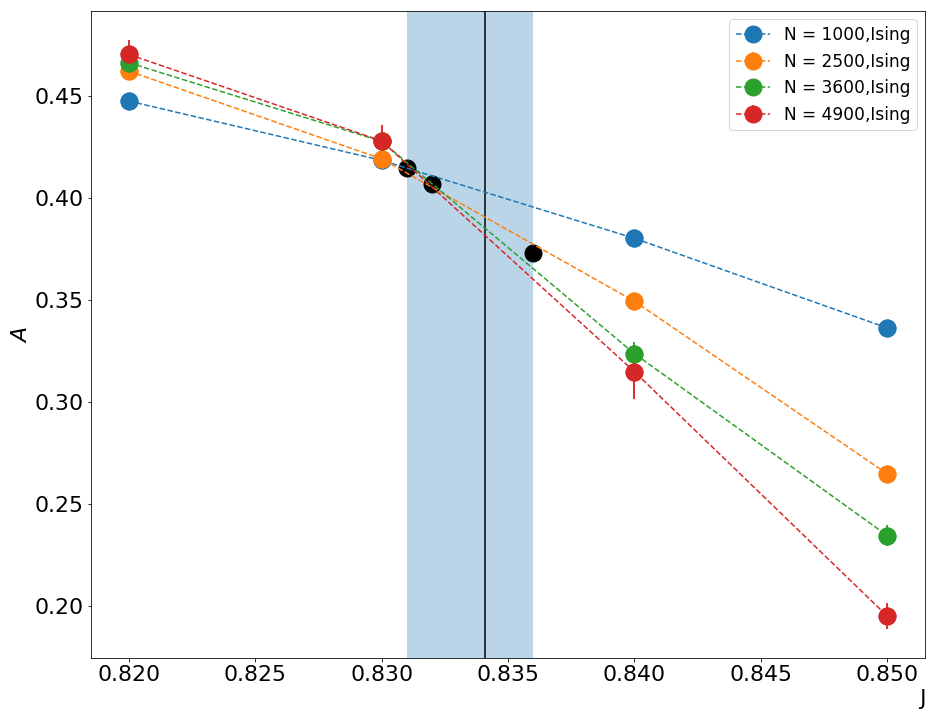
\includegraphics[width=\columnwidth]{Images/Ising_A_J_Close.png}
    \caption{Asphericity of Ising-ISAW model as function of zoomed in the critical region (red vertical lines), varying lengths of conformations N = 1000 (blue), 2500 (yellow), 3600 (green) and 4900 (red)}
    \label{fig:Ising_A_J}
\end{figure}

We took mean values of asphericity of Ising-ISAW model in the borders of critical region and in the point of the best crossing of plots where we observe phase transition according to our numerical results. All these points are marked as black in zoomed figures \ref{fig:Ising_A_J} and \ref{fig:ISAW_A_J}. Our following steps was to pick up values of aspect ratio, so the Rectangular Ising had the same asphericity and to enumerate critical cumulant of the model with the same shape factors. For simulations we used cluster update based on Wolff algorithm\cite{newmanb99}.

\begin{table}[h!]
    \centering
    \begin{tabular}{|c|c|c|c|}
        \hline
         \multicolumn{4}{|c|}{Ising-ISAW}  \\ \hline
         J & $\mathcal{A}$ & r & $U_{4}\  Rectangular$ \\ \hline
         0.831 & 0.415 & 0.465 & $0.340 \pm 0.006$\\ \hline
         0.832 & 0.4072 & 0.47 & $0.343 \pm 0.006$\\ \hline
         0.836 & 0.373 & $0.490 \pm 0.002$ & $0.348 \pm 0.006$\\ \hline
         \end{tabular}
    \caption{Values of critical cumulant for Ising model on rectangular lattice with mean asphericity related to Ising-ISAW model in its critical region}
    \label{tab:A_r_U}
\end{table}

As a result, comparison with critical cumulant of Ising-ISAW model, which was enumerated in \cite{faizullina2021critical} ($U_{4} = 0.308(8)$) showed significant mismatch of values, which means that we had not took into account some other geometrical properties - for example, which will be considered in the next part - proportions of monomers with different quantities of nearest neighbors. It is obvious that in Ising model on the rectangular lattice most of monomers located inside the lattice and have 4 nearest neighbors, while monomers spread around the perimeter of the lattice have at least 2 (corners) and 3 nearest neighbors. Proportions in Ising-ISAW conformations are completely different.

\subsection{Bulk}

\section{Discussion}

\section{Acknowledgments}

\bibliography{bibliography}

\end{document}